\subsection{Jugador (Player)}
\label{player}

\begin{figure}[H]
	\centering
	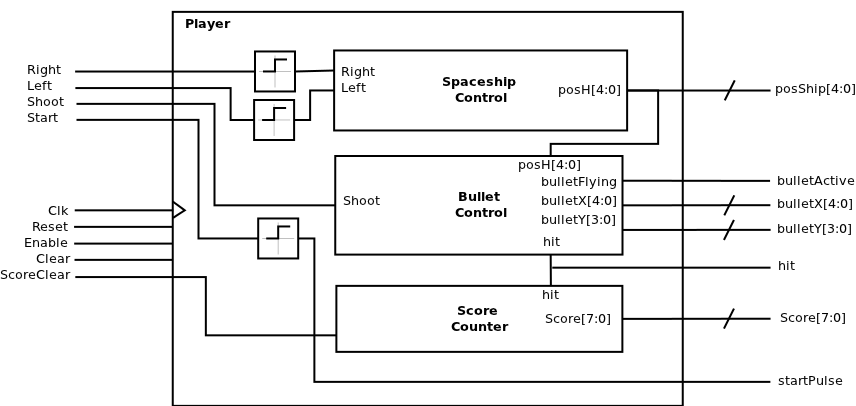
\includegraphics[width=0.6\textwidth]{player_block.png}
	\caption{Diagrama de bloques del Jugador (player) }\label{fig:playerBlock}
\end{figure}

Con el fin de agrupar todas las funciones de un jugador para mayor claridad, hemos creado un bloque Jugador (Player) que incluye toda la funcionalidad del jugador, de forma que además podemos instanciar varios jugadores de forma sencilla. Esto ha facilitado el añadir un segundo jugador a nuestro juego, simplemente instanciando este bloque 2 veces.

El bloque Jugador (figura \ref{fig:playerBlock}) incluye: tres detectores de flancos con antirrebote para las señales de movimiento a izquierda y derecha y de inicio, un control de la nave, un control del disparo y un contador para la puntuación.

También posee una serie de señales de control del bloque: Reset asíncrono, Clear síncrono ( pone todo a su estado inicial excepto la puntuación), un Clear síncrono para la puntuación y una entrada Enable para su habilitación, que afecta a todos los bloques excepto al detector de flancos de inicio, que siempre está activo.

La implementación en VHDL simplemente instancia los bloques necesarios y realiza las conexiones entre ellos. El contador de la puntación, sin embargo, se ha implementado como un proceso, que incrementa una unidad el contador cada vez que le llega una señal de marciano alcanzado por un disparo (hit).

